\section{Применение уравнений электростатики}

	Мы записали два уравнения:
	\begin{eqnarray}
		& \oint E_n \d{S}=\dfrac{q_{\Sigma}}{\varepsilon_0}, \\
		& \oint E_l \d{l}=0.
	\end{eqnarray}
	Сформулируем \i{принцип симметрии}\index{Принцип!симметрии}: если некоторая система зарядов переходит сама в себя при некотором преобразовании симметрии (поворот, сдвиг, отражение), то картина создаваемого поля переходит сам а в себя при этом преобразовании. \par

	Рассмотрим равномерно заряженную сферу \index{Сфера!заряженная} радиуса $R$. При повороте вокруг прямой $r$ вектор $\vec{E}$ переходит сам в себя. В каждой точке сферы радиуса $r$ поле \index{Поле} нормально и равно $E$, а 
	\begin{equation}
		\oint E_n \d{S}=E\cdot 4\pi r^2=\frac{q(r)}{\varepsilon_0},
	\end{equation}
	где $q(r)$ -- заряд внутри сферы радиуса $r$ с центром в той же точке. Отсюда
	\begin{equation}
		E=\frac{1}{4\pi r^2}\frac{q(r)}{\varepsilon_0}.
	\end{equation}
	Если $r<R$, то поле $E$ равно нулю, так как $q(r)=0$. При $r\qe R$ $q(r)=q$. Окончательно
	\begin{equation}
		E(r)=\begin{cases}
					0,& \text{$0\le r<R$},\\
					k\dfrac{q}{r^2},& \text{$r\qe R$}.
				\end{cases}
	\end{equation}
	\begin{figure}
		\centering
		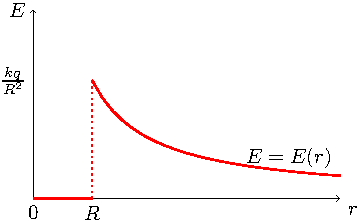
\includegraphics[scale=2]{./img/plot1/plot1.pdf}
		\caption{График поля в зависимости от расстояния $E=E(r)$ для однородно заряженной сферы}
	\end{figure}
	Для поля однородного шара запишем снова: $E(r)=k\dfrac{q(r)}{r^2}$. Поскольку шар заряжен равномерно, то
		$$\dfrac{q(r)}{q}=\frac{V(r)}{V}=\frac{r^3}{R^3},$$
	откуда
		$$q(r)=q\frac{r^3}{R^3},$$
	а
	\begin{equation}
		E(r)=\begin{cases}
					kq\dfrac{r}{R^3},& \text{$0\le r<R$},\\
					k\dfrac{q}{r^2},& \text{$r\qe R$}.
				\end{cases}
	\end{equation}
	\begin{figure}
		\centering
		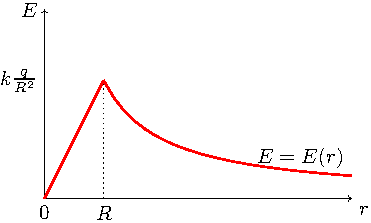
\includegraphics[scale=2]{./img/plot2/plot2.pdf}
		\caption{График поля в зависимости от расстояния $E=E(r)$ для однородно заряженного шара}
	\end{figure}